\documentclass[aspectratio=169]{beamer}

%https://en.wikibooks.org/wiki/LaTeX/Presentations
%\AtBeginSection[]{\subsection{}}
%\beamertemplatenavigationsymbolsempty

%\usetheme{Singapore}
%\usetheme{Rochester}
%\usetheme{JD}
%\usetheme{PaloAlto}
%\usetheme{Copenhagen}
%\usecolortheme{orchid}
%\usecolortheme{whale}

%\usecolortheme{Antibes}
\useoutertheme[hideothersubsections]{sidebar}
\usetheme{Rochester}
\usecolortheme{orchid}
\useoutertheme[hideothersubsections]{sidebar}
\setbeamertemplate{itemize items}[circle]
\setbeamertemplate{section in toc}[circle]

%\usepackage{helvet}


\title
    [Main Project]
    {Multi-core RISC Processor Design \& Implementation}
\subtitle{Demonstration Viva}

\author
    [B. Lancaster]
    {Ben Lancaster}
\institute
    [\hypersetup{urlcolor=jdgrey}%
     \href{https://bendl.me/}{https://bendl.me}
    ]
    {201280376\\
    ELEC5881M - Main Project}
\date
    [12/2016]
    {\today}



\begin{document}

\begin{frame}[plain]
\titlepage
\end{frame}

\begin{frame}
\tableofcontents
\end{frame}

\section{Introduction}
\frame{\tableofcontents[currentsection, subsectionstyle=show/show/hide]}

\subsection{Why Multi-core?}
\begin{frame}{Why Multi-core?}
\begin{alertblock}{Block Title}
Lorem ipsum dolor sit amet, consectetur adipisicing elit, 
sed do eiusmod tempor incididunt ut labore et 
dolore magna aliqua.
\end{alertblock}
\end{frame}

\subsection{Why RISC?}
\begin{frame}{Why RISC?}
\end{frame}

\section{Top Level Design}
\frame{\tableofcontents[currentsection, subsectionstyle=show/show/hide]}

\subsection{Overview}
\begin{frame}{Overview}
\textbf{What this project produces:}
\begin{itemize}[<+->]\setlength\itemsep{1em}
    \item{\textbf{System-on-Chip with multi-processor functionality}\\
    Tested on FPGA hardware with 1-96 CPU cores.}
    \item{\textbf{Custom 16-bit RISC CPU}\\
    With interrupts and its own Instruction Set Architecture (ISA).}
    \item{\textbf{Aimed at Design Engineers, not end users}\\
    Project is provided as source code/design files for Design Engineers to customise and implement in hardware themselves.}
    \item{\textbf{Software/Assembly compiler}\\
    PRCO304 programming language/Intel assembly syntax.}
\end{itemize}
\end{frame}

\begin{frame}{Top Level Hierarchy}
\begin{figure}
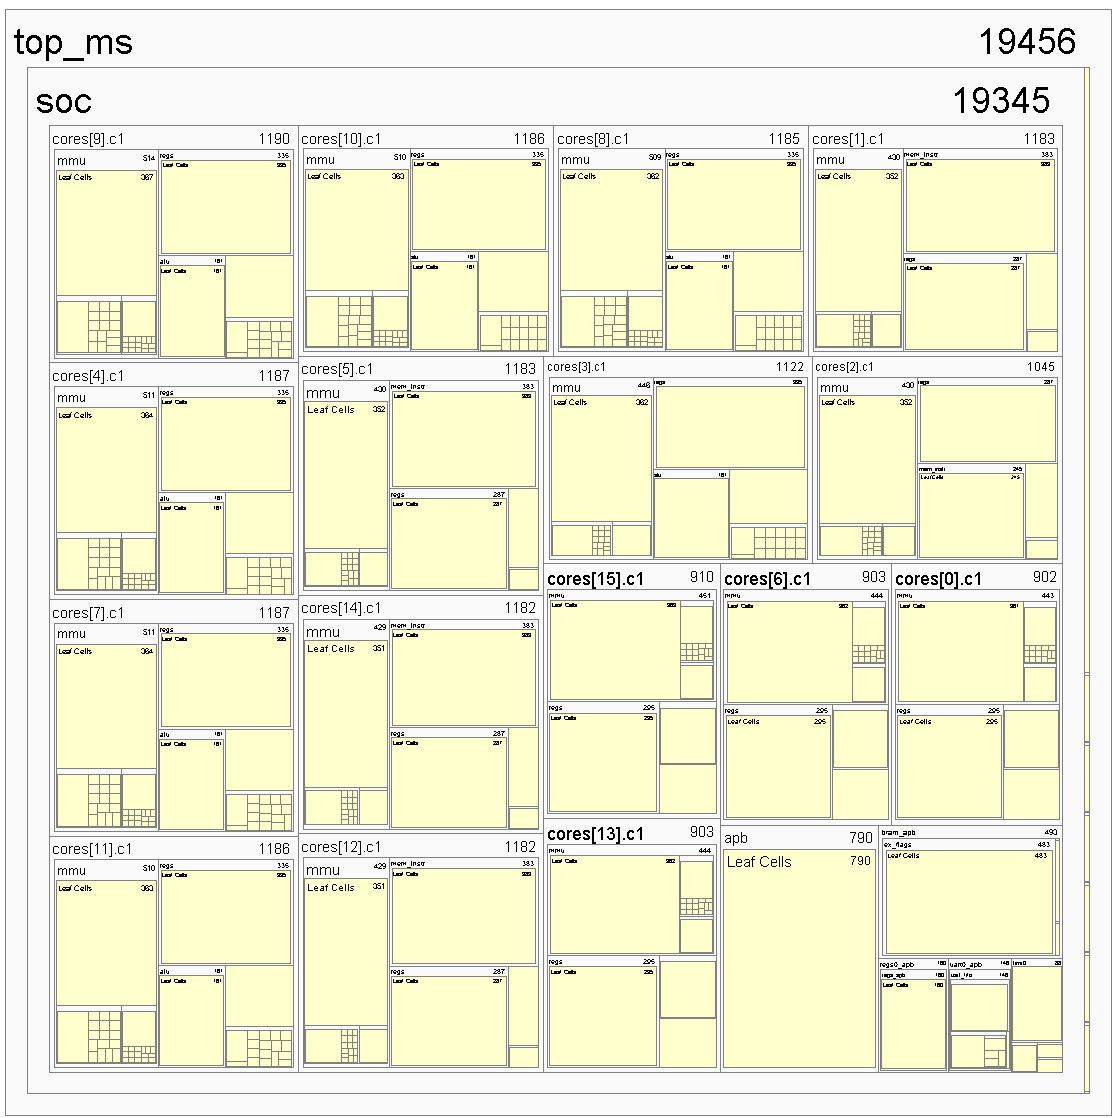
\includegraphics[width=7cm]{soc_layout_schem}
\end{figure}
\end{frame}

\subsection{Memory Map}
\begin{frame}{Memory Map}
\begin{columns}
\column{0.5\textwidth}
\begin{figure}
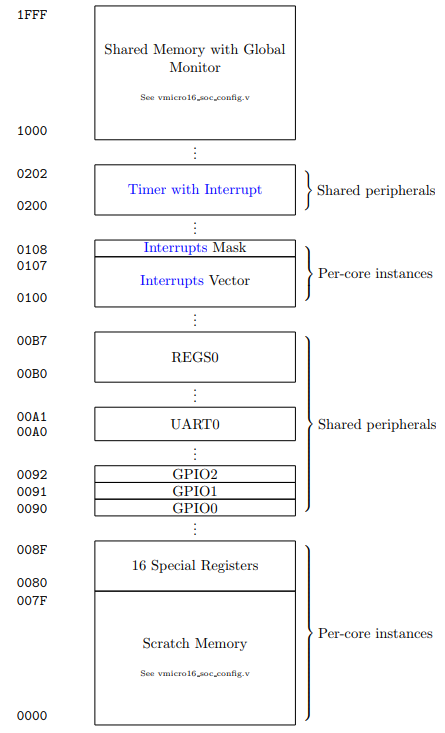
\includegraphics[width=4cm]{memory_map}
\end{figure}
\column{0.5\textwidth}
\begin{itemize}
    \item \textbf{Shared Memory with Global Monitor}
    \item Timer with Interrupt
    \item Per-core Interrupt Vector and Mask
    \item Shared Register Set
    \item UART Transceiver
    \item Multiple GPIO ports
    \item Per-core scratch memory
    \item \textbf{Per-core Special Registers}
    \item Customisable by designers
\end{itemize}
\end{columns}
\end{frame}

\subsection{Interrupts}
\begin{frame}{Interrupts}
\end{frame}

\subsection{Interconnect}
\begin{frame}{Interconnect}
\end{frame}

\section{Multi-core Functionality}
\frame{\tableofcontents[currentsection, subsectionstyle=show/show/hide]}
\subsection{HW/SW Requirements}
\begin{frame}{HW/SW Requirements}
\begin{columns}[t]
\column{0.5\textwidth}
Hardware:
\begin{itemize}
    \item Bus Arbitration/Scheduling\\ (priority, rotating, etc.)
    \item Atomic functions\\ (atomic versions of load-
\end{itemize}
\column{0.5\textwidth}
Software:
\begin{itemize}
    \item \textbf{Shared Memory with Global Monitor}
    \item Timer with Interrupt
    \item Per-core Interrupt Vector and Mask
    \item Shared Register Set
    \item UART Transceiver
    \item Multiple GPIO ports
    \item Per-core scratch memory
    \item \textbf{Per-core Special Registers}
    \item Customisable by designers
\end{itemize}
\end{columns}

\end{frame}

\section{Results}
\frame{\tableofcontents[currentsection, subsectionstyle=show/show/hide]}
\begin{frame}{Results}
\end{frame}
\subsection{Results 1}
\begin{frame}{Results 1}
\end{frame}

\section{Conclusion}
\frame{\tableofcontents[currentsection, subsectionstyle=show/show/hide]}
\begin{frame}{Conclusion}
\end{frame}

\end{document}
